\documentclass[12pt]{article}
\usepackage[utf8]{inputenc}
\usepackage[greek,english]{babel}
\usepackage{alphabeta}
\usepackage{fancyhdr}
\usepackage{listings}
\usepackage{mathtools}
\usepackage{xcolor}
\usepackage{float}
\usepackage{siunitx}
\usepackage[margin=0.5in]{geometry}
\usepackage[backend=bibtex]{biblatex}

\lstset {
        basicstyle=\ttfamily,
        columns=fullflexible,
        breaklines=true,
        keepspaces=true,
	showstringspaces=false
}

\title{Εργαστήριο Ασφάλειας στην Τεχνολογία της Πληροφορίας -- Εργασία 5}
\author{Χρήστος Μαργιώλης -- 19390133}
\date{Ιούνιος 2023}

\begin{document}

\begin{titlepage}
        \maketitle
        \begin{figure}[t!]
        \begin{center}
        
\includegraphics[scale=0.3]{./res/uniwalogo.png} \\
        \Large
        \textbf{Πανεπιστήμιο Δυτικής Αττικής} \\
        \large
        Τμήμα Μηχανικών Πληροφορικής και Ηλεκτρονικών Υπολογιστών
        \end{center}
        \end{figure}
\end{titlepage}

\renewcommand{\contentsname}{Περιεχόμενα}
\tableofcontents
\pagebreak

\section{Εργαλεία}

Τα δύο εργαλεία που χρησιμοποιήθηκαν για την εργασία είναι το
\begin{itemize}
	\item \lstinline{https://www.ssllabs.com/ssltest}
	\item \lstinline{https://www.sslshopper.com/ssl-checker.html}
\end{itemize}

Το πρώτο εργαλείο πραγματοποιεί αρκετά πιο εκτενείς ελέγχους.

\section{'Ασκηση 1}

Το ηλεκτρονικό μαγαζί που θα ελεγχθεί είναι το skroutz.gr.

\subsection{Εργαλείο 1}

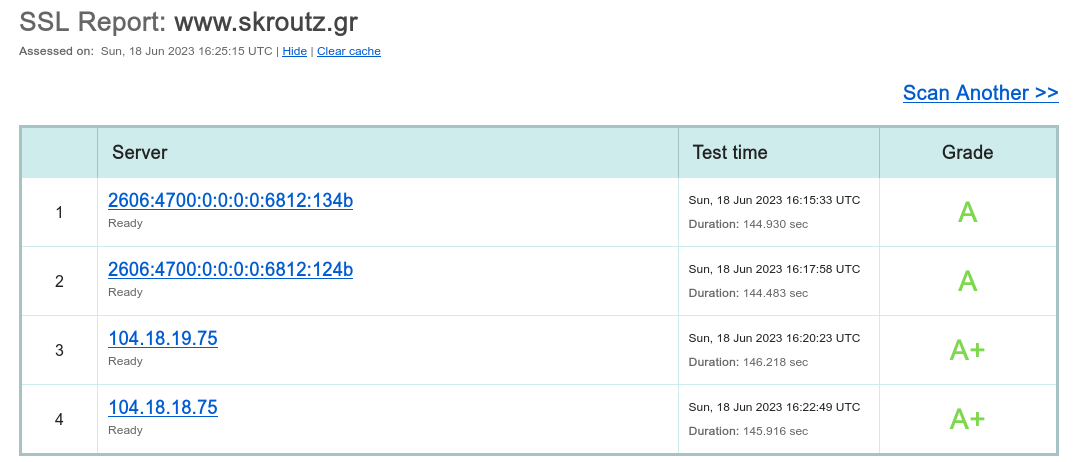
\includegraphics[width=\textwidth]{res/skroutz1.png} \\

\subsection{Εργαλείο 2}

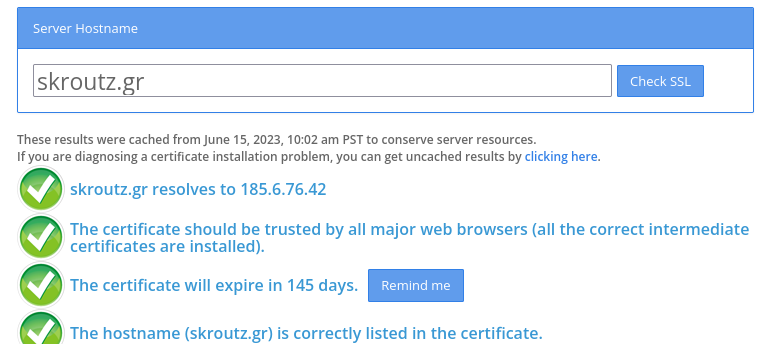
\includegraphics[width=\textwidth]{res/skroutz2.png} \\

\section{'Ασκηση 2}

Η ειδησεογραφική σελίδα που θα ελεγχθεί είναι το CNN. 

\subsection{Εργαλείο 1}

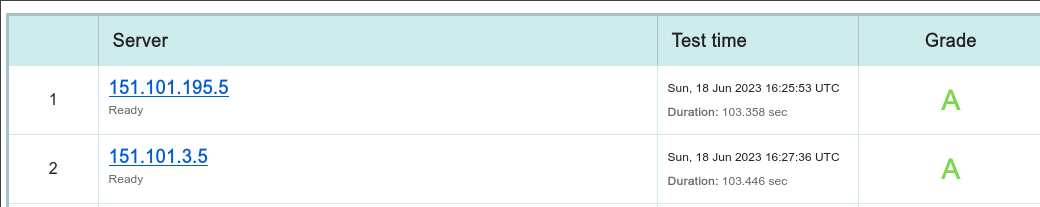
\includegraphics[width=\textwidth]{res/cnn1.png} \\

\subsection{Εργαλείο 2}

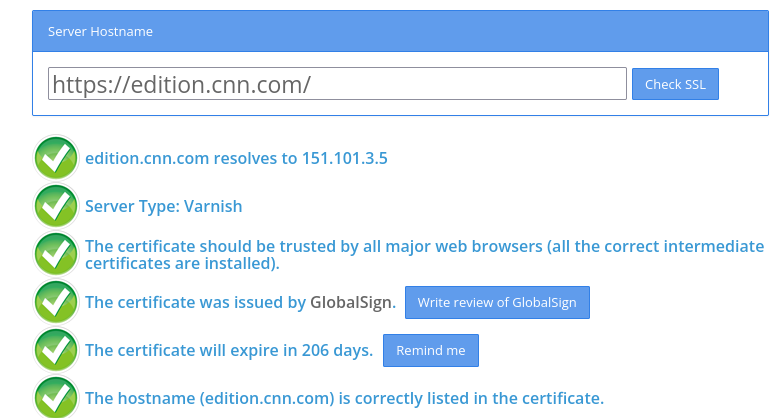
\includegraphics[width=\textwidth]{res/cnn2.png} \\

\section{'Ασκηση 3}

Η πανεπιστημιακή σελίδα που θα ελεγχθεί είναι το uniwa.gr. 

\subsection{Εργαλείο 1}

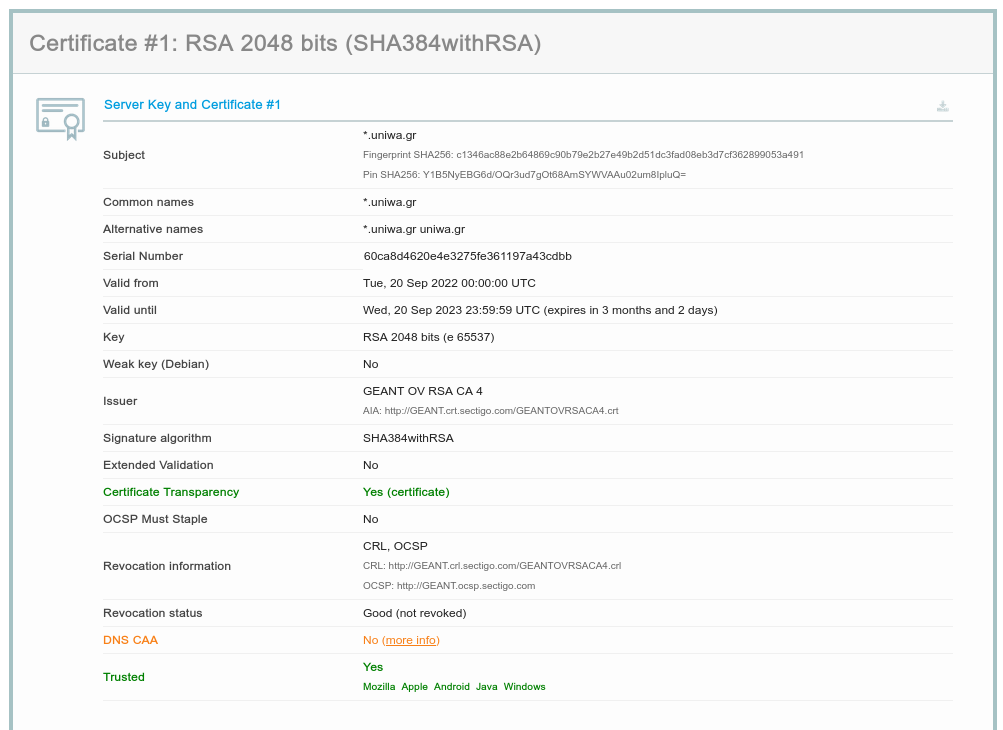
\includegraphics[width=\textwidth]{res/uniwa1.png} \\

\subsection{Εργαλείο 2}

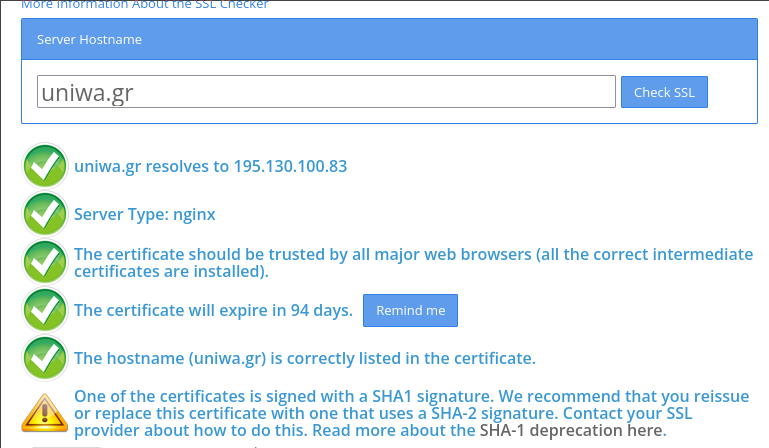
\includegraphics[width=\textwidth]{res/uniwa2.png} \\

\end{document}
